\documentclass{report}
\usepackage{graphicx}
\usepackage{csvsimple}
\usepackage[T5]{fontenc}
\usepackage[a4paper, top=2cm, bottom=2cm, left=2cm, right=2cm]{geometry}

\renewcommand{\thesection}{\arabic{section}}

\begin{document}

\begin{titlepage}
    \center
    \LARGE{Vietnam Posts and Telecommunications Institute of Technology (PTIT)} \\
    \vspace*{\fill}
    
    
\includegraphics[scale=0.5]{ptit-logo.png} \\
    \vspace{1cm}
    \huge\textbf{Python 2nd Assignment \\ Image Classification} \\
    \vspace{1cm}

    \Large
    \begin{tabular}{@{}lll@{}}
    Students: & Trần, Vũ Tiến Minh & B23DCCE067 \\
              & Phạm, Quốc Hùng    & B23DCVT188 \\
    Lecturer: & Dr. Kim, Ngọc Bách &            \\
    Class:    & D23CQCE04-B        &            \\
    Date:     & \today             &            \\  
    \end{tabular}

    \vspace{\fill}
\end{titlepage}

\chapter*{Introduction}
This report is the justification and the results of the assignment. The assignment focuses on building, training and 
testing two simple neural networks to classify the CIFAR-10 dataset: A three layers Multi-Layer Perceptron 
(MLP) and a three convolution layers Convolutional Neural Network (CNN).

\section*{The Assignment Tasks}
These are the main tasks:
\begin{itemize}
    \item Build a basic MLP (Multi-Layer Perceptron) neural network with 3 layers.
    \item Build a Convolutional Neural Network (CNN) with 3 convolution layers.
    \item Perform image classification using both neural networks, including training, validation, and testing.
    \item Plot learning curves.
    \item Plot confusion matrix.
    \item Use the PyTorch library.
\end{itemize}

\section*{Package Dependencies}
These packages are centered around working with the PyTorch library as the requirement has stated:
\begin{itemize}
    \item \texttt{torch}: For building and training neural networks.
    \item \texttt{torchvision}: For getting datasets and image transformations.
    \item \texttt{scikit-learn}: For train/validation splitting and calculating confusion matrix.
    \item \texttt{numpy}: For numerical operations.
    \item \texttt{matplotlib}: For plotting learning curves, confusion matrices and others.
\end{itemize}

\newpage
\tableofcontents
\newpage

\chapter*{Report}

\section{CIFAR-10 Dataset}
CIFAR-10 dataset is a well-known dataset for image classification exercise. It has 60,000, $32\times32$ pixels images 
in 10 classes, with 6,000 images per class. PyTorch library splits the dataset into 50,000 training images and 
10,000 testing images. 

\begin{figure}[ht]
    \center
    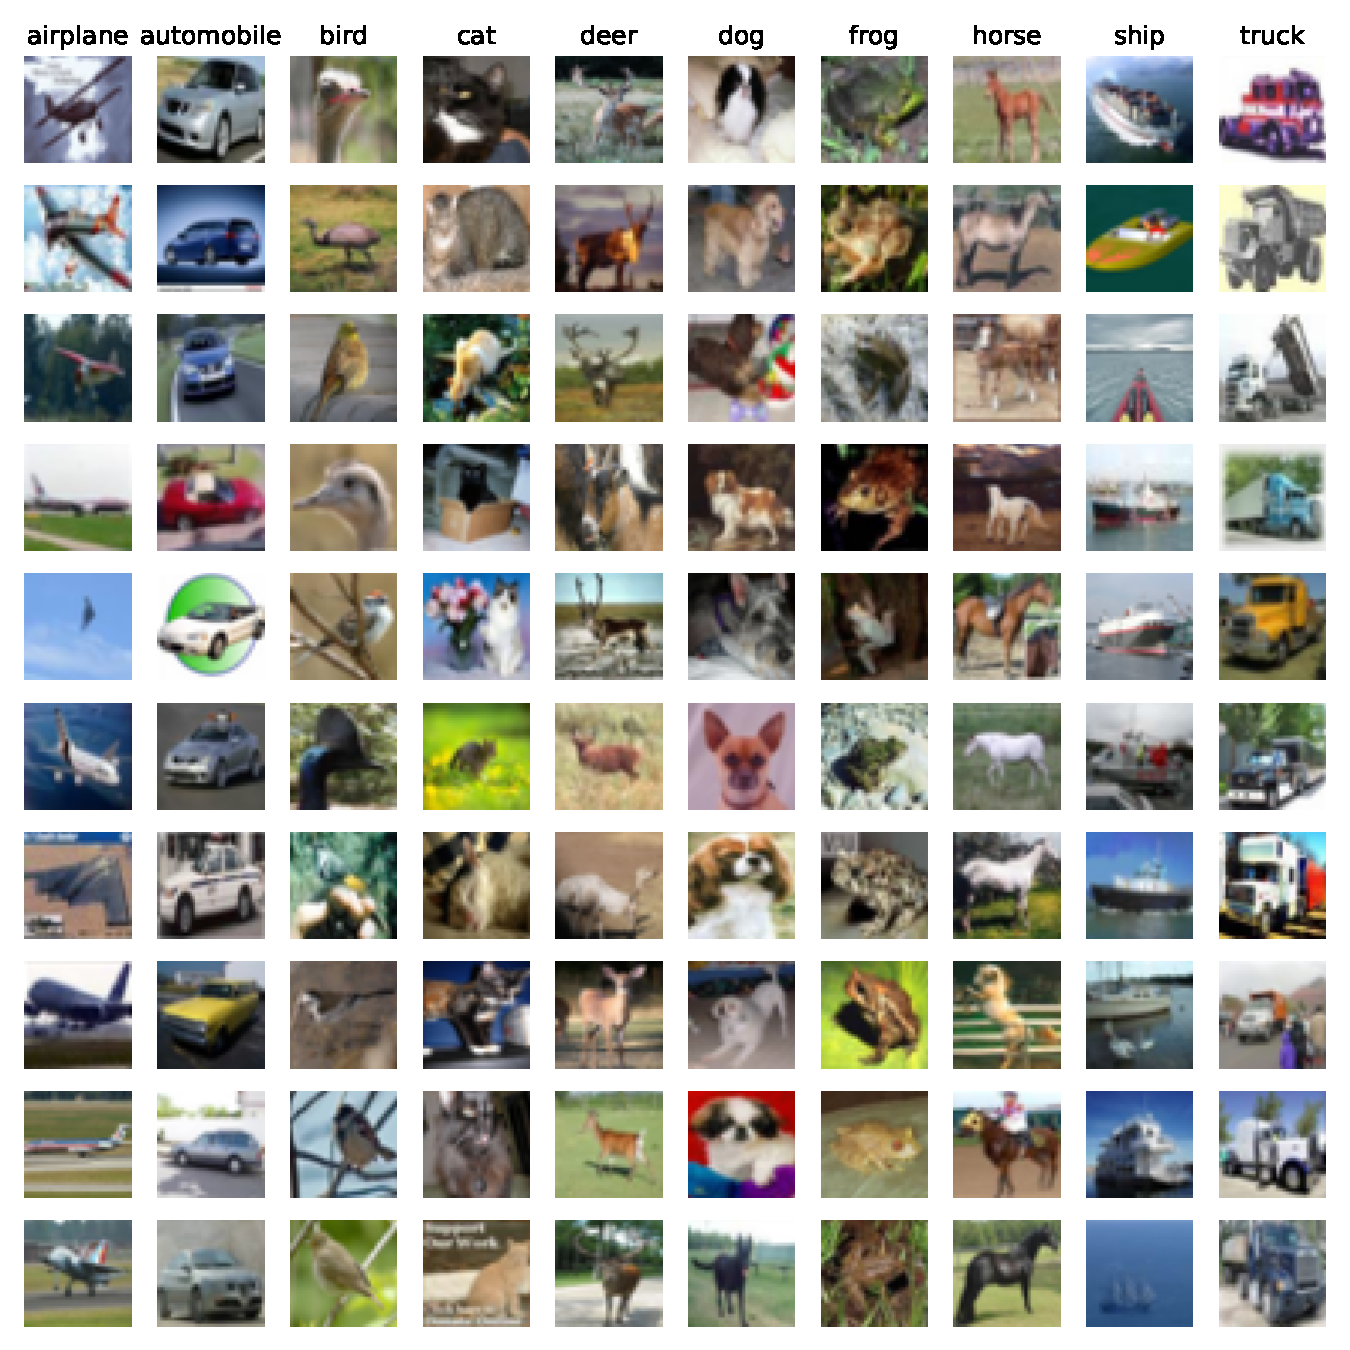
\includegraphics[scale=0.7]{../output/cifar10-images.pdf}
    \caption{cifar10-images.pdf}
\end{figure}

In this project, to do training validation and testing seperately, the 50.000 images set is split into 40,000 
training images and 10,000 validation images. This is a common method of tuning the model based on the validation 
set's results, and then testing the model with the test set to have an unbiased evaluation of the model.

\section{Data Analysis}
The first step of any Machine Learning exercise is to do Data Analysis. All analysis will be done on the 40,000 
images train set only. This is to simulate the real world scenario, where the test set is not available during the 
training process. The validation set is solely used for tuning the model, so it is not used in the analysis.

\subsection{Color Distribution} 
The below graphs show the RGB color distribution of the dataset, with the color intensity ranging from 0 to 
255. Based on the graph, all three channels does follow a balanced distribution to some degree, minus the very 
high peak at the 250 region. The blue channel specifically is right skewed, so unlike other distribution with a 
mean around 128, blue has a mean around 100.

\begin{figure}[ht]
    \center
    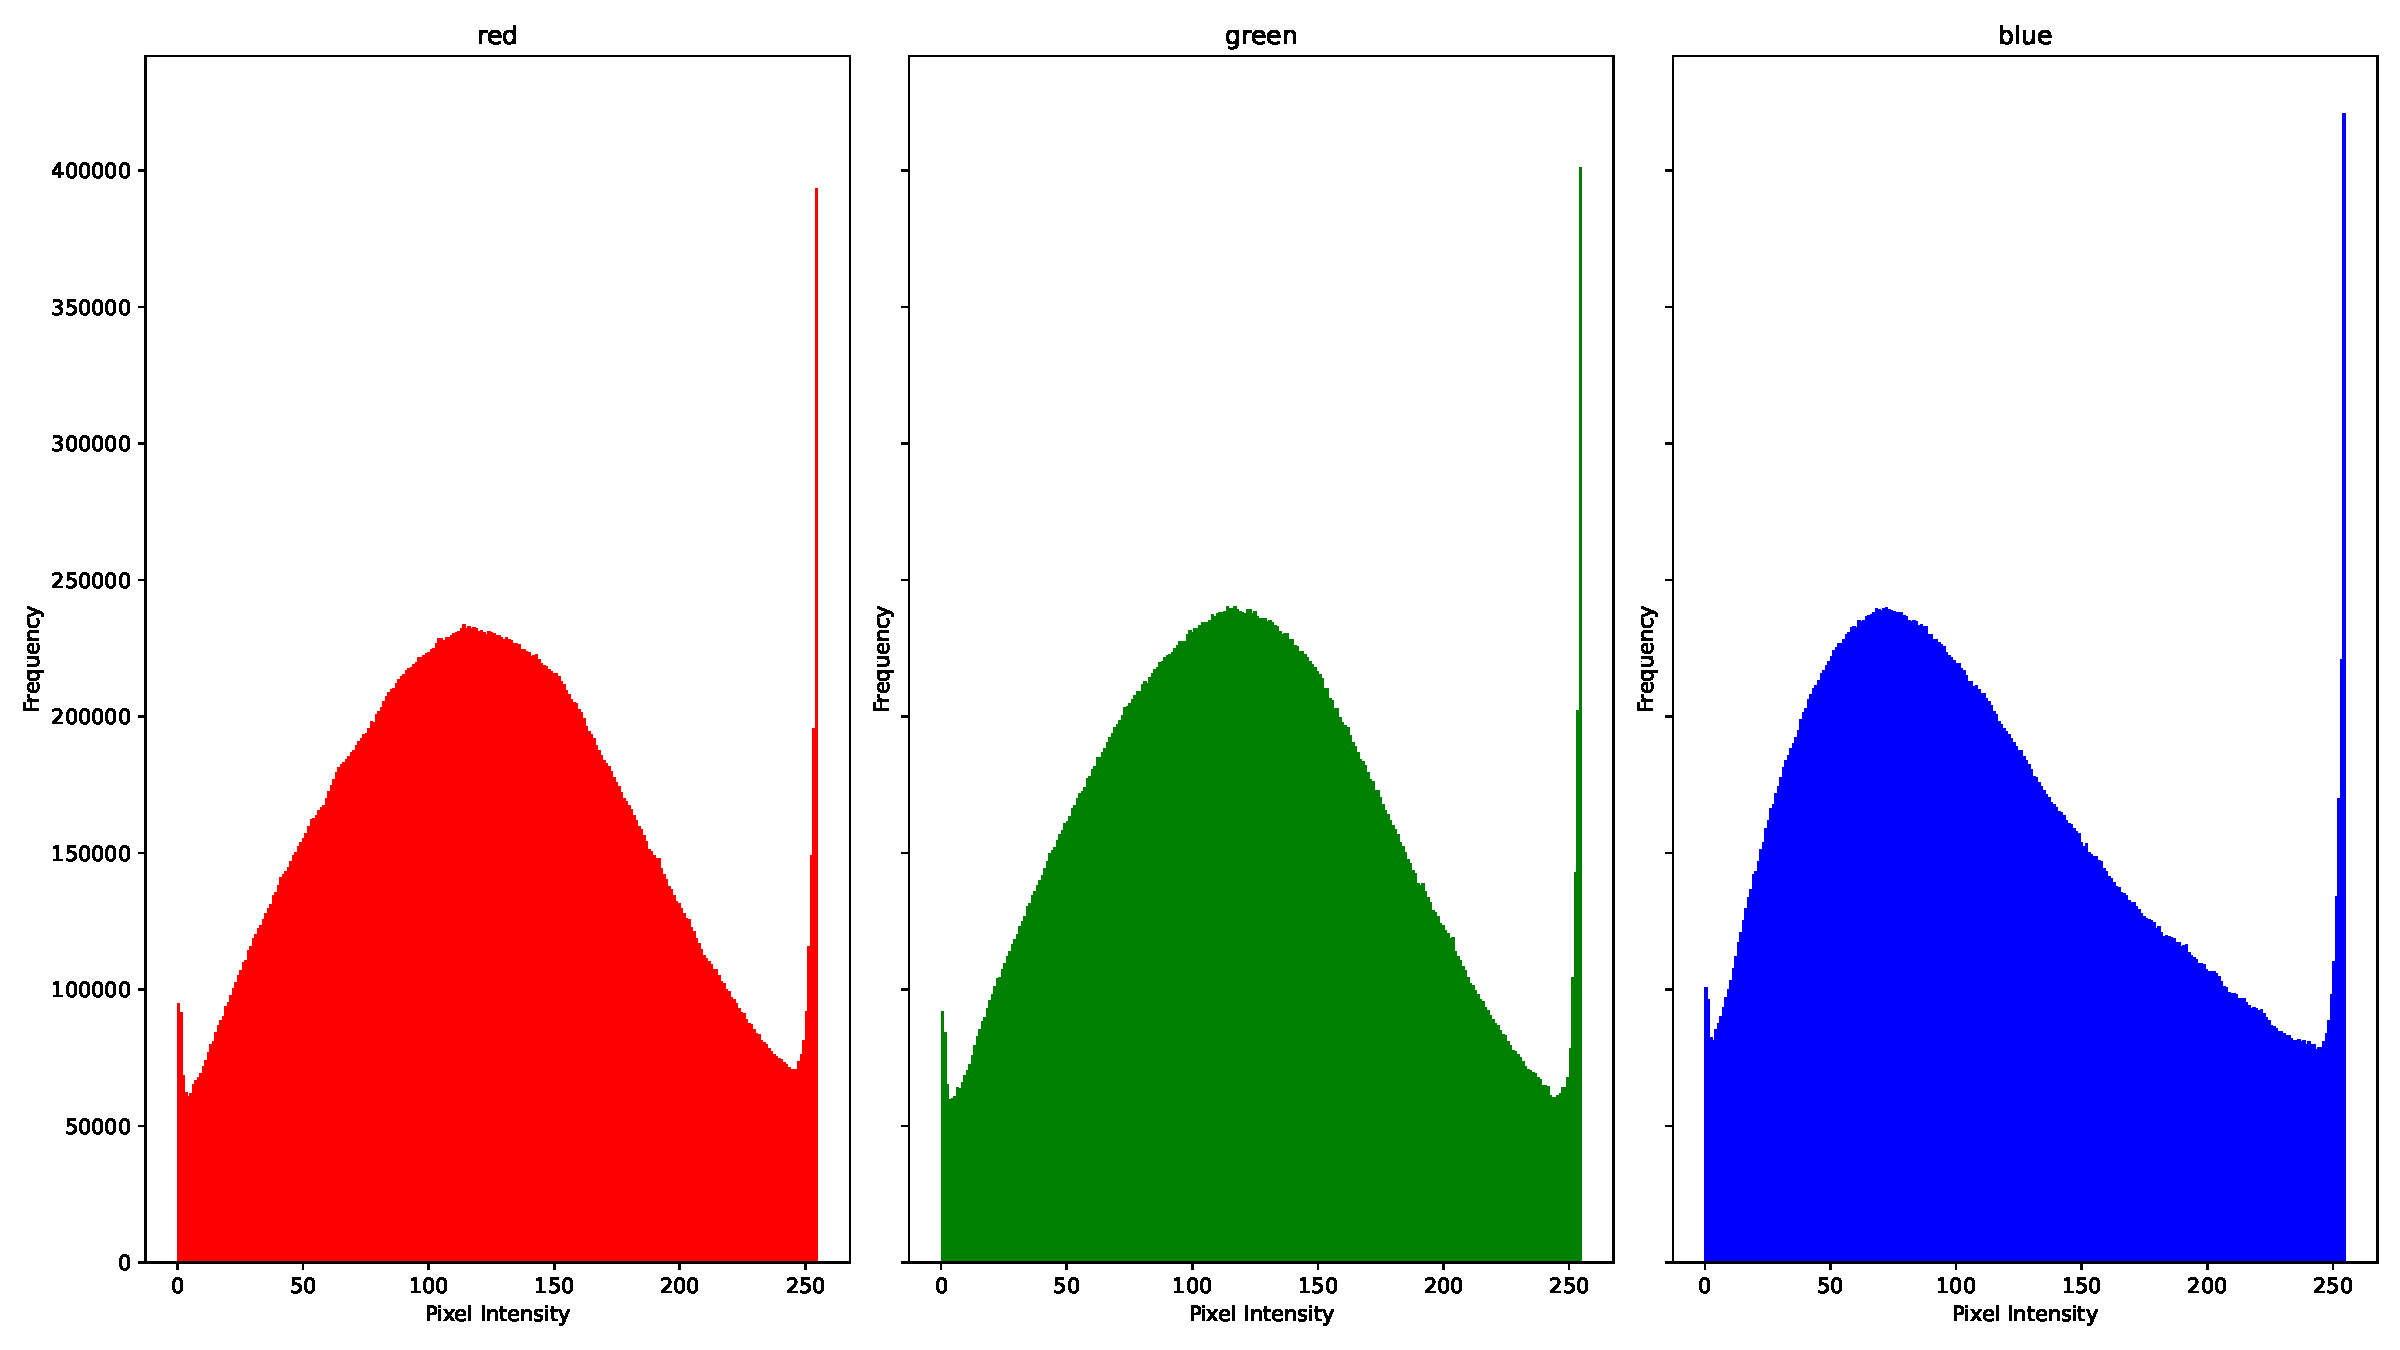
\includegraphics[scale=0.4]{../output/cifar10-channels.pdf}
    \caption{cifar10-channels.pdf}
\end{figure}

\subsection{Mean And Standard Deviation} 
MLP and CNN can perform better on a normalized dataset, resulting in a faster convergence and better accuracy. 
In PyTorch, the \texttt{torchvision.transforms.Normalize} function normalizes images by adjusting their pixel 
values according to the mean and standard deviation of the dataset. The table below includes the raw values 
and also the normalized values divided by 255.

\begin{table}[ht]
    \center
    \csvautotabular{../output/cifar10-mean-std.csv}
    \caption{cifar10-mean-std.csv}
\end{table}

\subsection{Transforming The Dataset}
Before normalization, all three datasets are converted .\texttt{torchvision.transforms.ToTensor}, each image is 
reshaped from a dimension of $32\times32\times3$ to $3\times32\times32$.

\newpage
\begin{verbatim}
    # python
    from torchvision import transforms

    transform = transforms.Compose([
        transforms.ToTensor(),
        transforms.Normalize(mean, std)
    ])
\end{verbatim}

\section{Building Models}
To keep the project simple, both models' hyper parameters were tuned by hand after each training/validation 
cycle until the performance is deemed high enough. Below are the final structure of the two models.

\subsection{Multi-Layer Perceptron}
The MLP model used for this assignment consists of three fully connected linear layers:

\begin{verbatim}
    # python
    from torch import nn

    relu = nn.ReLU()
    dropout = nn.Dropout(0.2)
    
    model = nn.Sequential(                  # (_, 3, 32, 32)
        nn.Flatten(),                       # (_, 3 * 32 * 32)

        nn.Linear(3 * 32 * 32, 512),        # (_, 512)
        nn.BatchNorm1d(512),
        relu,
        dropout,

        nn.Linear(512, 256),                # (_, 256)
        nn.BatchNorm1d(256),
        relu,
        dropout,

        nn.Linear(256, 10)                  # (_, 10)
    )
\end{verbatim}

\begin{enumerate}
    \item \textbf{Flatten Layer:} Converts the input image into a 1D vector.
    \item \textbf{First Linear Block:}
    \begin{itemize}
        \item Fully connected layer with 512 output units.
        \item Batch normalization for improved training stability.
        \item ReLU activation for non-linearity.
        \item Dropout 20\% for regularization.
    \end{itemize}
    \item \textbf{Second Linear Block:}
    \begin{itemize}
        \item Fully connected layer with 256 output units.
        \item Batch normalization.
        \item ReLU activation.
        \item Dropout 20\%.
    \end{itemize}
    \item \textbf{Output Linear Layer:} Fully connected layer mapping to 10 output classes.
\end{enumerate}

\subsection{Convolutional Neural Network}
The CNN model used for this assignment consists of three convolution layers and one output linear layer:

\begin{verbatim}
    # python
    from torch import nn

    relu = nn.ReLU()
    maxpool = nn.MaxPool2d(2, stride=2)
    dropout = nn.Dropout2d(0.2)

    model = nn.Sequential(                  # (_, 3, 32, 32)
        nn.Conv2d(3, 128, 3, padding=1),    # (_, 128, 32, 32)
        nn.BatchNorm2d(128),
        relu,
        maxpool,                            # (_, 128, 16, 16)
        dropout,

        nn.Conv2d(128, 256, 3, padding=1),  # (_, 256, 16, 16)
        nn.BatchNorm2d(256),
        relu,
        maxpool,                            # (_, 256, 8, 8)
        dropout,

        nn.Conv2d(256, 512, 3, padding=1),  # (_, 512, 8, 8)
        nn.BatchNorm2d(512),
        relu,
        maxpool,                            # (_, 512, 4, 4)
        dropout,

        nn.Flatten(),                       # (_, 512 * 4 * 4)
        nn.Linear(512 * 4 * 4, 10)          # (_, 10)
    )
\end{verbatim}

\begin{enumerate}
    \item \textbf{First Convolutional Block:}
    \begin{itemize}
        \item 2D convolution: 3 input channels, 128 output channels, $3\times3$ kernel, padding=1. The padding=1 is 
              for preserving the dimensions from $30\times30$ to $32\times32$.
        \item Batch normalization.
        \item ReLU activation.
        \item $2\times2$ Max pooling reduces size to $16\times16$.
        \item Dropout 20\%.
    \end{itemize}
    \item \textbf{Second Convolutional Block:}
    \begin{itemize}
        \item 2D convolution: 128 input to 256 output channels.
        \item Batch normalization.
        \item ReLU activation.
        \item $2\times2$ Max pooling for size of $8\times8$.
        \item Dropout 20\%.
    \end{itemize}
    \item \textbf{Third Convolutional Block:}
    \begin{itemize}
        \item 2D convolution: 256 input to 512 output channels.
        \item Batch normalization.
        \item ReLU activation.
        \item $2\times2$ Max pooling for size of $4\times4$.
        \item Dropout 20\%.
    \end{itemize}
    \item \textbf{Output Linear Layer:}
    \begin{itemize}
        \item Flatten layer converts feature maps to a vector size of $512\times4\times4$.
        \item Fully connected linear layer mapping to 10 output classes.
    \end{itemize}
\end{enumerate}

\section{Criterion and Optimizers}
Now comes the most important part of the exercise: Optimize the optimizers. The two models use the same loss 
function \texttt{torch.nn.CrossEntropyLoss}. For the optimizer, MLP uses \texttt{torch.optim.AdamW} and CNN 
uses \texttt{torch.optim.SGD}. Similar to building the models, the optimizers' parameters were manually 
tuned after each validation cycle.

\subsection{Cross Entropy Loss}
\texttt{torch.nn.CrossEntropyLoss} is a loss function commonly used for multi-class classification problems, making 
it suitable for CIFAR-10. It is a combination of \texttt{torch.nn.LogSoftmax}, an activation function and 
\texttt{torch.nn.NLLLoss}, a loss function. \texttt{LogSoftmax} converts raw output scores into probabilities that sum to 
1 then apply logarithm. \texttt{NLLLoss} takes the log-probabilities and measures how far off the predictions are from 
the true labels. 

\[ L(x, y) = - \sum_{i=1}^{C} y_i \cdot \log(x_i) \]

\begin{center}
    \begin{tabular}{ll}
        $C$: & Number of classes  \\    
        $x$: & Predicted labels   \\
        $y$: & True labels        \\
    \end{tabular}
\end{center}

\subsection{Adaptive Moment Estimation With Weight}
\texttt{torch.optim.AdamW} is \texttt{torch.optim.Adam} with weight decay added. Adam by itself is a popular optimization 
algorithm combining the advantages of two other optimizers: \texttt{torch.optim.Adagrad} and \texttt{torch.optim.RMSprop}. 
Because of its adaptive nature, AdamW works well with its default hyper parameters. The final tuned weight decay is set to 
$10^{-3}$ to prevent MLP from over fitting.

\[
\begin{array}{rcl}
    m_t       & = & \beta_1 m_{t-1} + (1 - \beta_1) g_t                                 \\ [0.2cm]
    v_t       & = & \beta_2 v_{t-1} + (1 - \beta_2) g_t^2                               \\ [0.2cm]
    \hat{m}_t & = & \frac{m_t}{1 - \beta_1^t}                                           \\ [0.2cm]
    \hat{v}_t & = & \frac{v_t}{1 - \beta_2^t}                                           \\ [0.2cm]
    \theta_t  & = & \theta_{t-1} - \eta \left( \frac{\hat{m}_t}{\sqrt{\hat{v}_t} 
                    + \epsilon} + \lambda \theta_{t-1} \right)                             
\end{array}
\]

\begin{center}
    \begin{tabular}{ll}
        $g_t$:                    & Loss function's gradient at step t  \\
        $m_t$, $v_t$:             & 1st, 2nd moment estimates           \\
        $\hat{m}_t$, $\hat{v}_t$: & Bias-corrected of $m_t$, $v_t$      \\
        $\beta_1$, $\beta_2$:     & Decay rates of $m_t$, $v_t$         \\
        $\theta_t$:               & Model's parameters                  \\
        $\eta$:                   & Learning rate                       \\
        $\lambda$:                & Weight decay coefficient            \\
        $\epsilon$:               & Constant for numerical stability    
    \end{tabular}   
\end{center}

\subsection{Stochastic Gradient Descent}
\texttt{torch.optim.SGD} is one of the most commonly used optimization algorithms. It updates CNN parameters
using loss function's gradient. "Stochastic" means the gradients is from computing random mini batch rather 
than the whole dataset, making the process faster and more memory efficient. CNN is often paired with SGD 
+ momentum for better generalization. Although SGD requires more tuning, the performance gains can be 
significant. The momentum factor helps escape local minima and accelerates progress in shallow valleys. In the 
project, the final tuned parameters are: learning rate = 0.01, momentum = 0.9 and weight delay = $10^{-3}$.

\[
\begin{array}{rcl}
    v_{t+1}      & = & \mu v_t - \eta g_t                               \\ [0.2cm]
    g_t          & = & \nabla_{\theta} J(\theta_t) + \lambda \theta_t   \\ [0.2cm]
    \theta_{t+1} & = & \theta_t + v_{t+1}  
\end{array}
\]

\begin{center}
    \begin{tabular}{ll}
        $\theta_t$: & Model's parameters at step t      \\
        $\eta$:     & Learning rate                     \\
        $\lambda$:  & Weight decay coefficient          \\
        $\mu$:      & Momentum factor                   \\
        $v_t$:      & Velocity                          \\
        $g_t$:      & Gradient 
    \end{tabular}   
\end{center}

\section{Training And Validation}
\subsection{The Method}
With all the components ready, the training and validation process starts with spliting the two's dataset into 
smaller batches. Aside from reducing hardware workload, smaller train batches leads to faster parameter updates 
and improve generalization. Batches too small can introduce noises, slowing down convergence while too large 
gives a smoother params updates but less generalization. The training batch size in the project is set to 64 
after some tuning, that is a total of 625 batches from 40,000 images. For the validation set, the batch size is 
1,000 because the dataset is used for tuning parameters, not training.  

\begin{verbatim}
    # python

    model = ...
    train_losses = []
    train_accuracies = []
    validation_losses = []
    validation_accuracies = []

    for epoch in range(20):
        train_loss, train_accuracy = train(model, train_loader)
        validation_loss, validation_accuracy = test(model, validation_loader)

        train_losses.extend(train_loss)
        train_accuracies.extend(train_accuracy)
        validation_losses.append(validation_loss)
        validation_accuracies.append(validation_accuracy)
\end{verbatim}

Both models will train through the train dataset 20 times (20 epochs). The training loss and accuracy values 
are calculated after every 25 batches trained for a more detailed reference for parameters tuning. The validation 
values are calculated after each training cycle.

\subsection{Learning Curve}
Based on the validation values collected above, a learning curve graph can be plotted to show some insights on 
how well tuned are the parameters.

\subsubsection*{Underfitting}
\begin{itemize}
    \item Training loss is high
    \item Validation loss is also high
    \item Accuracy is low for both
\end{itemize}
This means model is learning too slowly. In this case, increase the number of epochs or the learning rate factor.

\subsubsection*{Overfitting}
\begin{itemize}
    \item Training loss is low, accuracy is high
    \item Validation loss is high, accuracy is low
\end{itemize}
This means model fits training data well but doesn't generalize. In this case, increase the optimizer's weight
delay or the model's dropout parameter. Or maybe this is the best that the model can do, consider an early stopping.

\newpage
The below graphs are the learning curves of two models after some tuning. MLP validation loss and accuracy
come to a hault at the 10th epoch with the accuracy around 55\%. This is expected considering MLPs 
usually struggle on image data compared to CNN. On the other side, CNN performs exceptionally well with the
validation accuracy at 80\% and is still rising slowly. 

\begin{figure}[ht]
    \center
    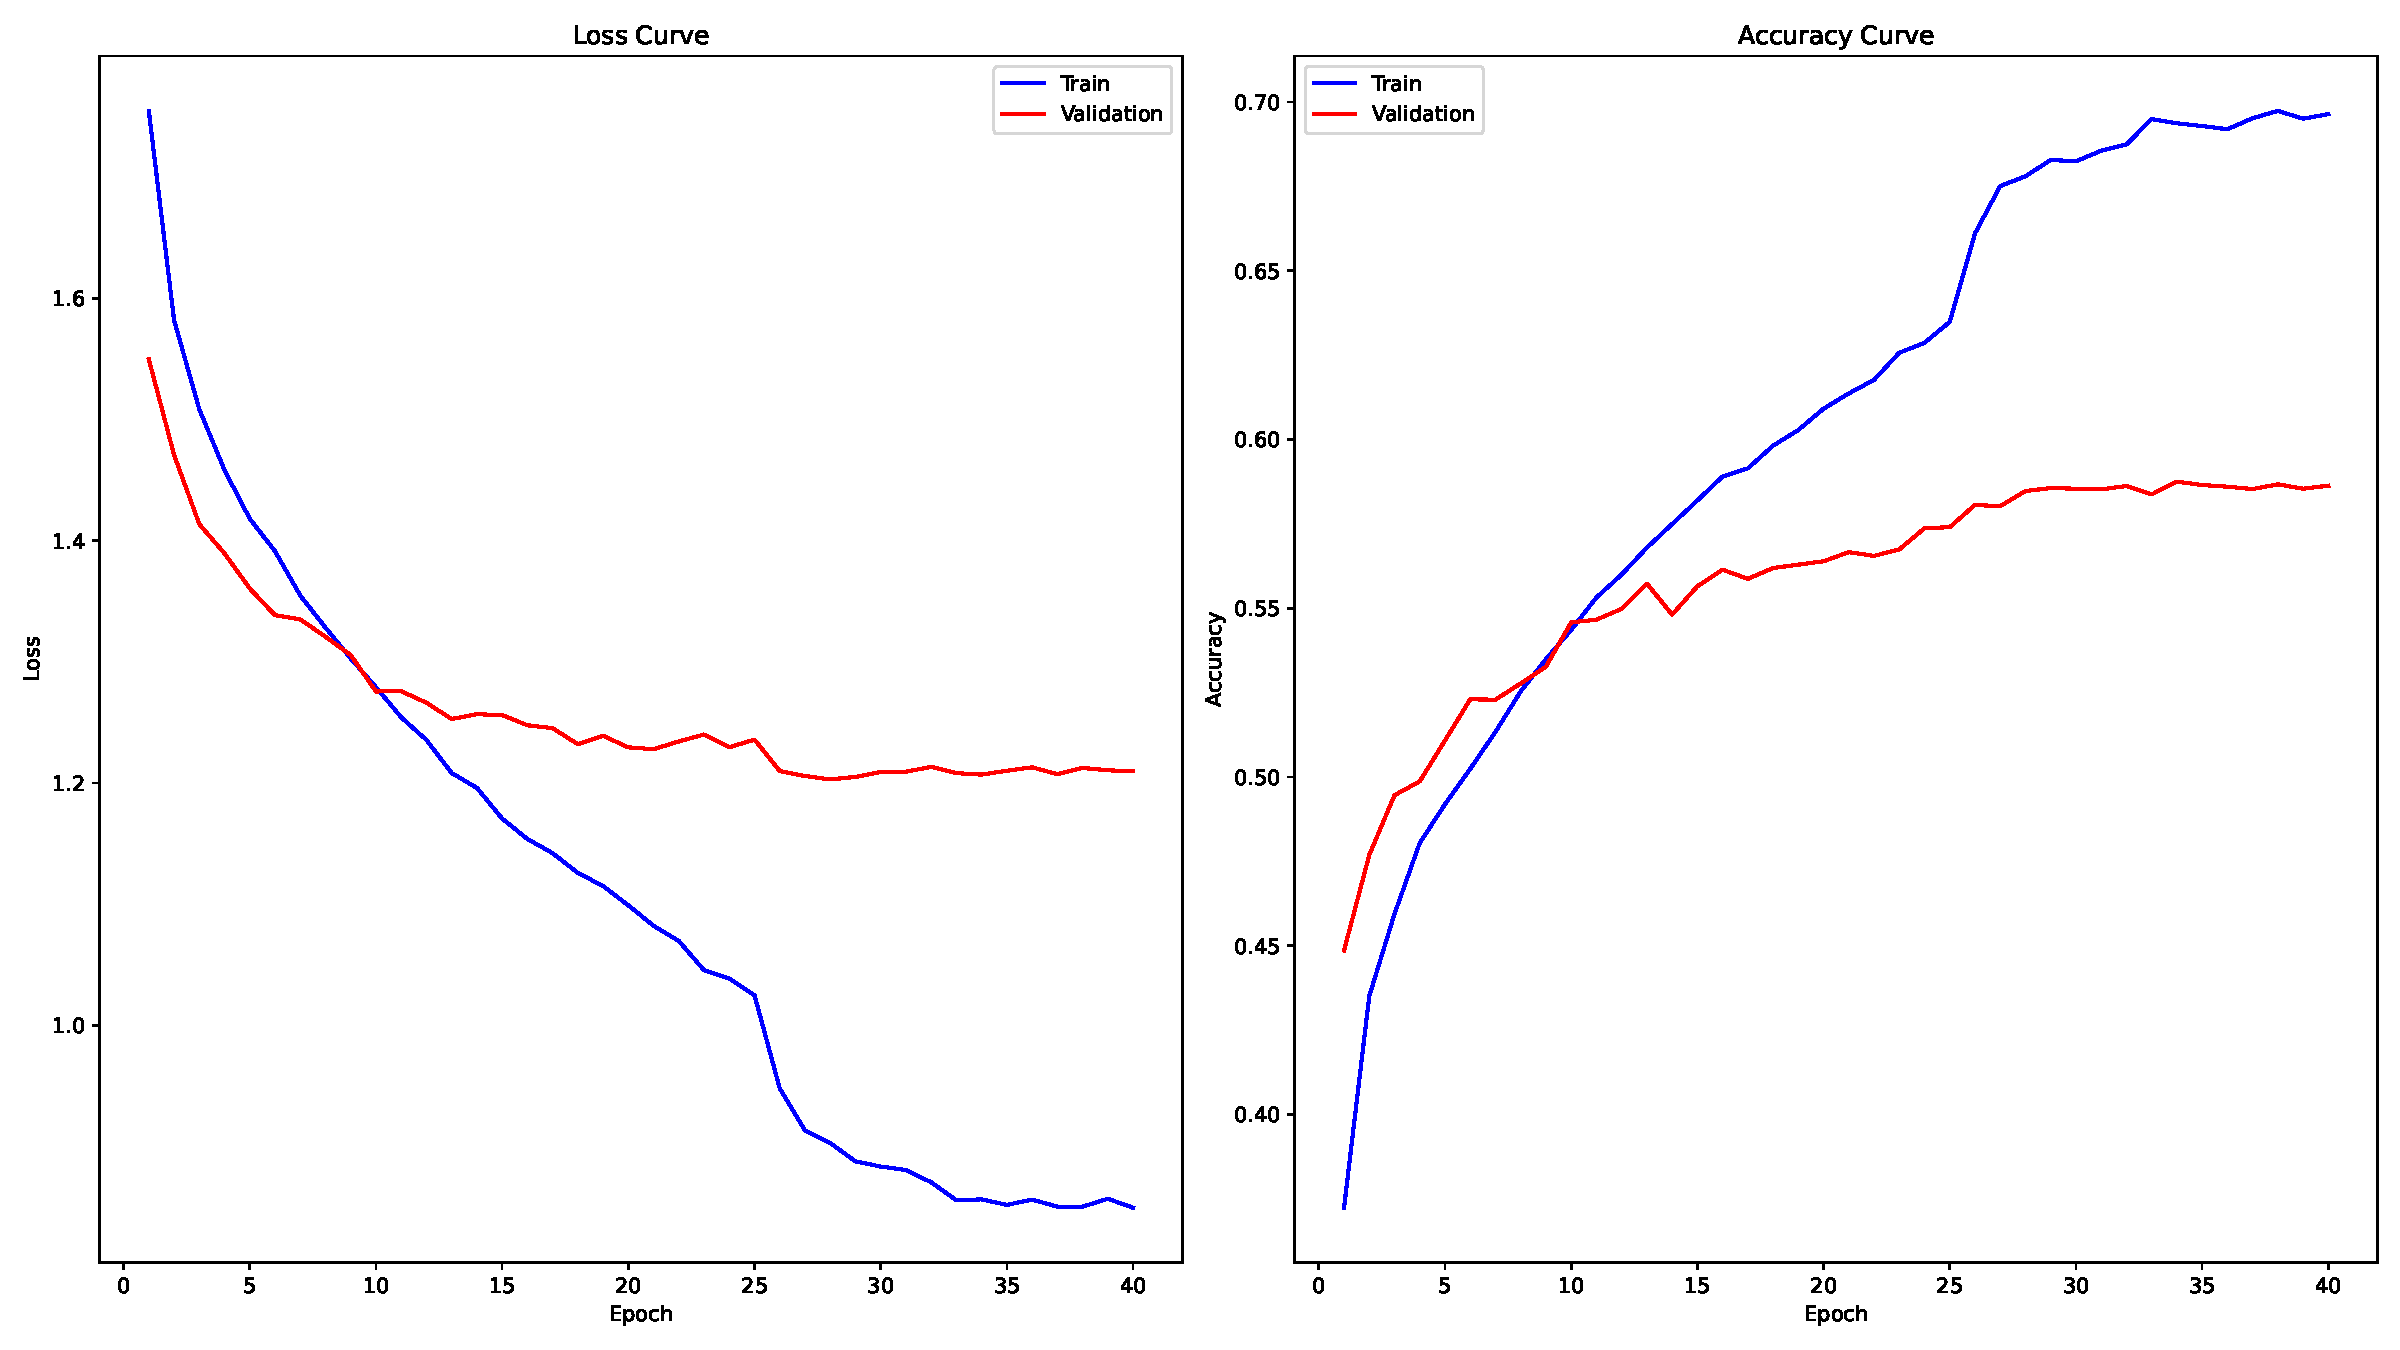
\includegraphics[scale=0.385]{../output/mlp-learning-curve.pdf}
    \caption{mlp-learning-curve.pdf}
\end{figure}

\begin{figure}[ht]
    \center
    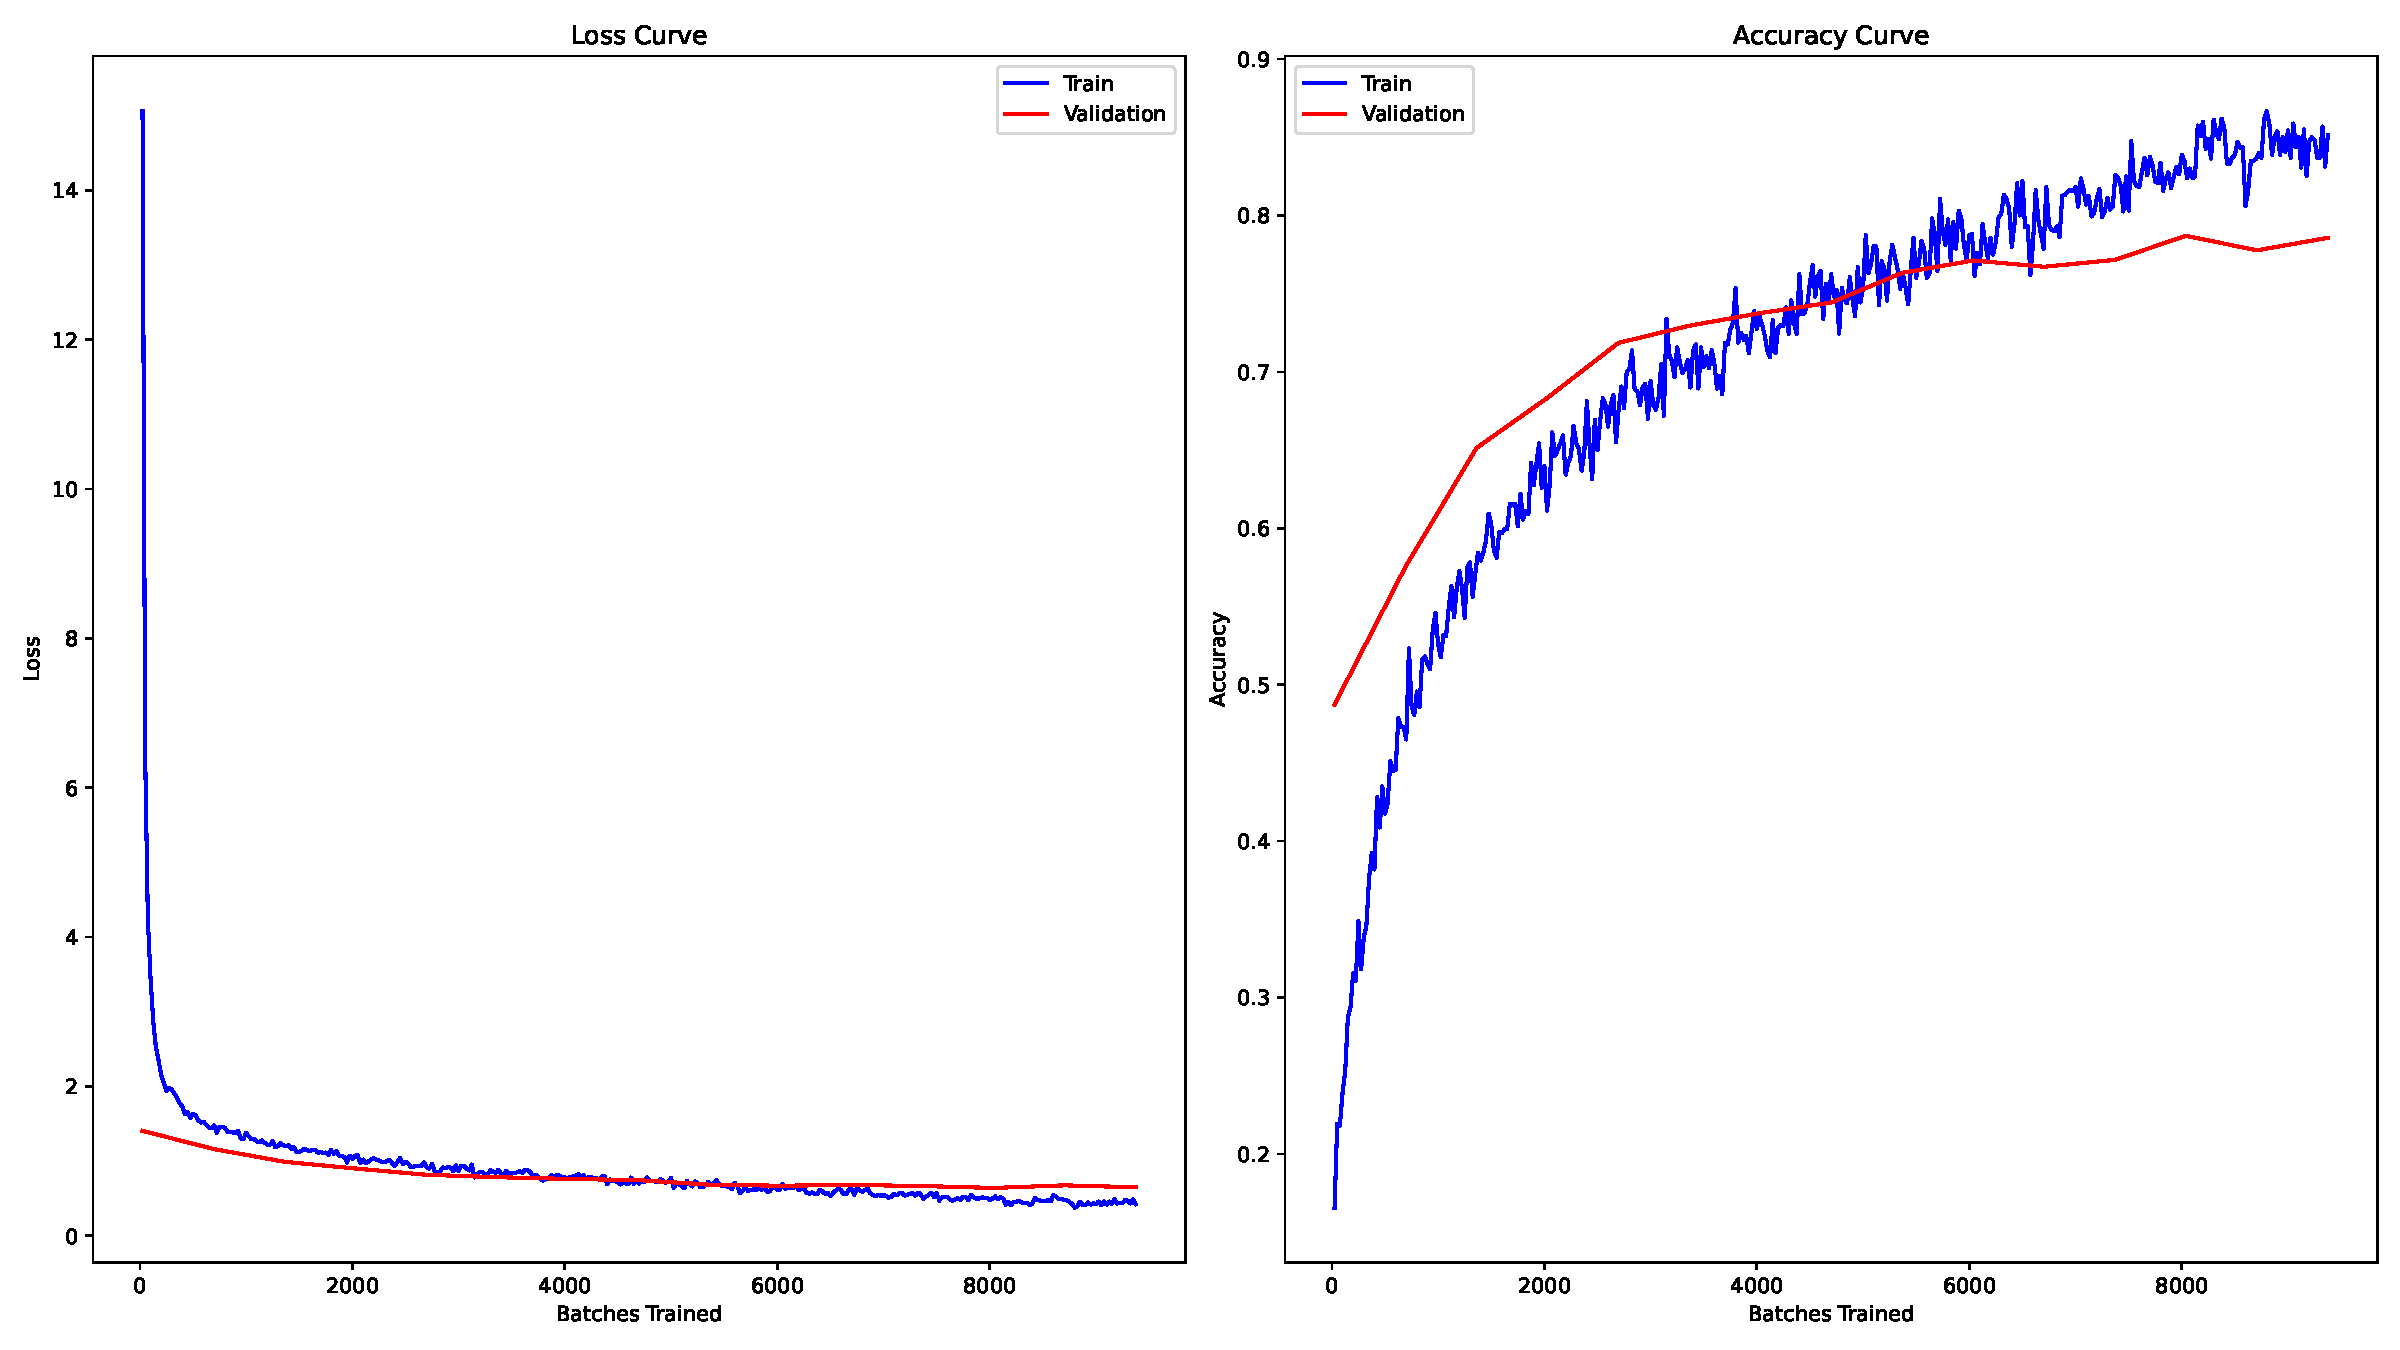
\includegraphics[scale=0.385]{../output/cnn-learning-curve.pdf}
    \caption{cnn-learning-curve.pdf}
\end{figure}

\newpage
\section{Testing Results}
To evaluate the two trained models without any bias, the final step is to run the models through unseen data, 
which is the testing dataset. Below are the losses, accuracies and confusion matrices. The loss and accuracy 
values are identical to the validation dataset, which implies that the validation method is well fitted for this task. 
The Confusion matrices help visualize where are the hotspots of misprediction at. Both models find difficulties differentiating 
between cats and dogs, automobiles and trucks, ships and airplanes. Unlike CNN, MLP hotspots spread out more inside the two class 
groups: the animal classes and the vehicle group. However, MLP recognises well if the data is an animal or a vehicle.

\begin{figure}[ht]
    \center
    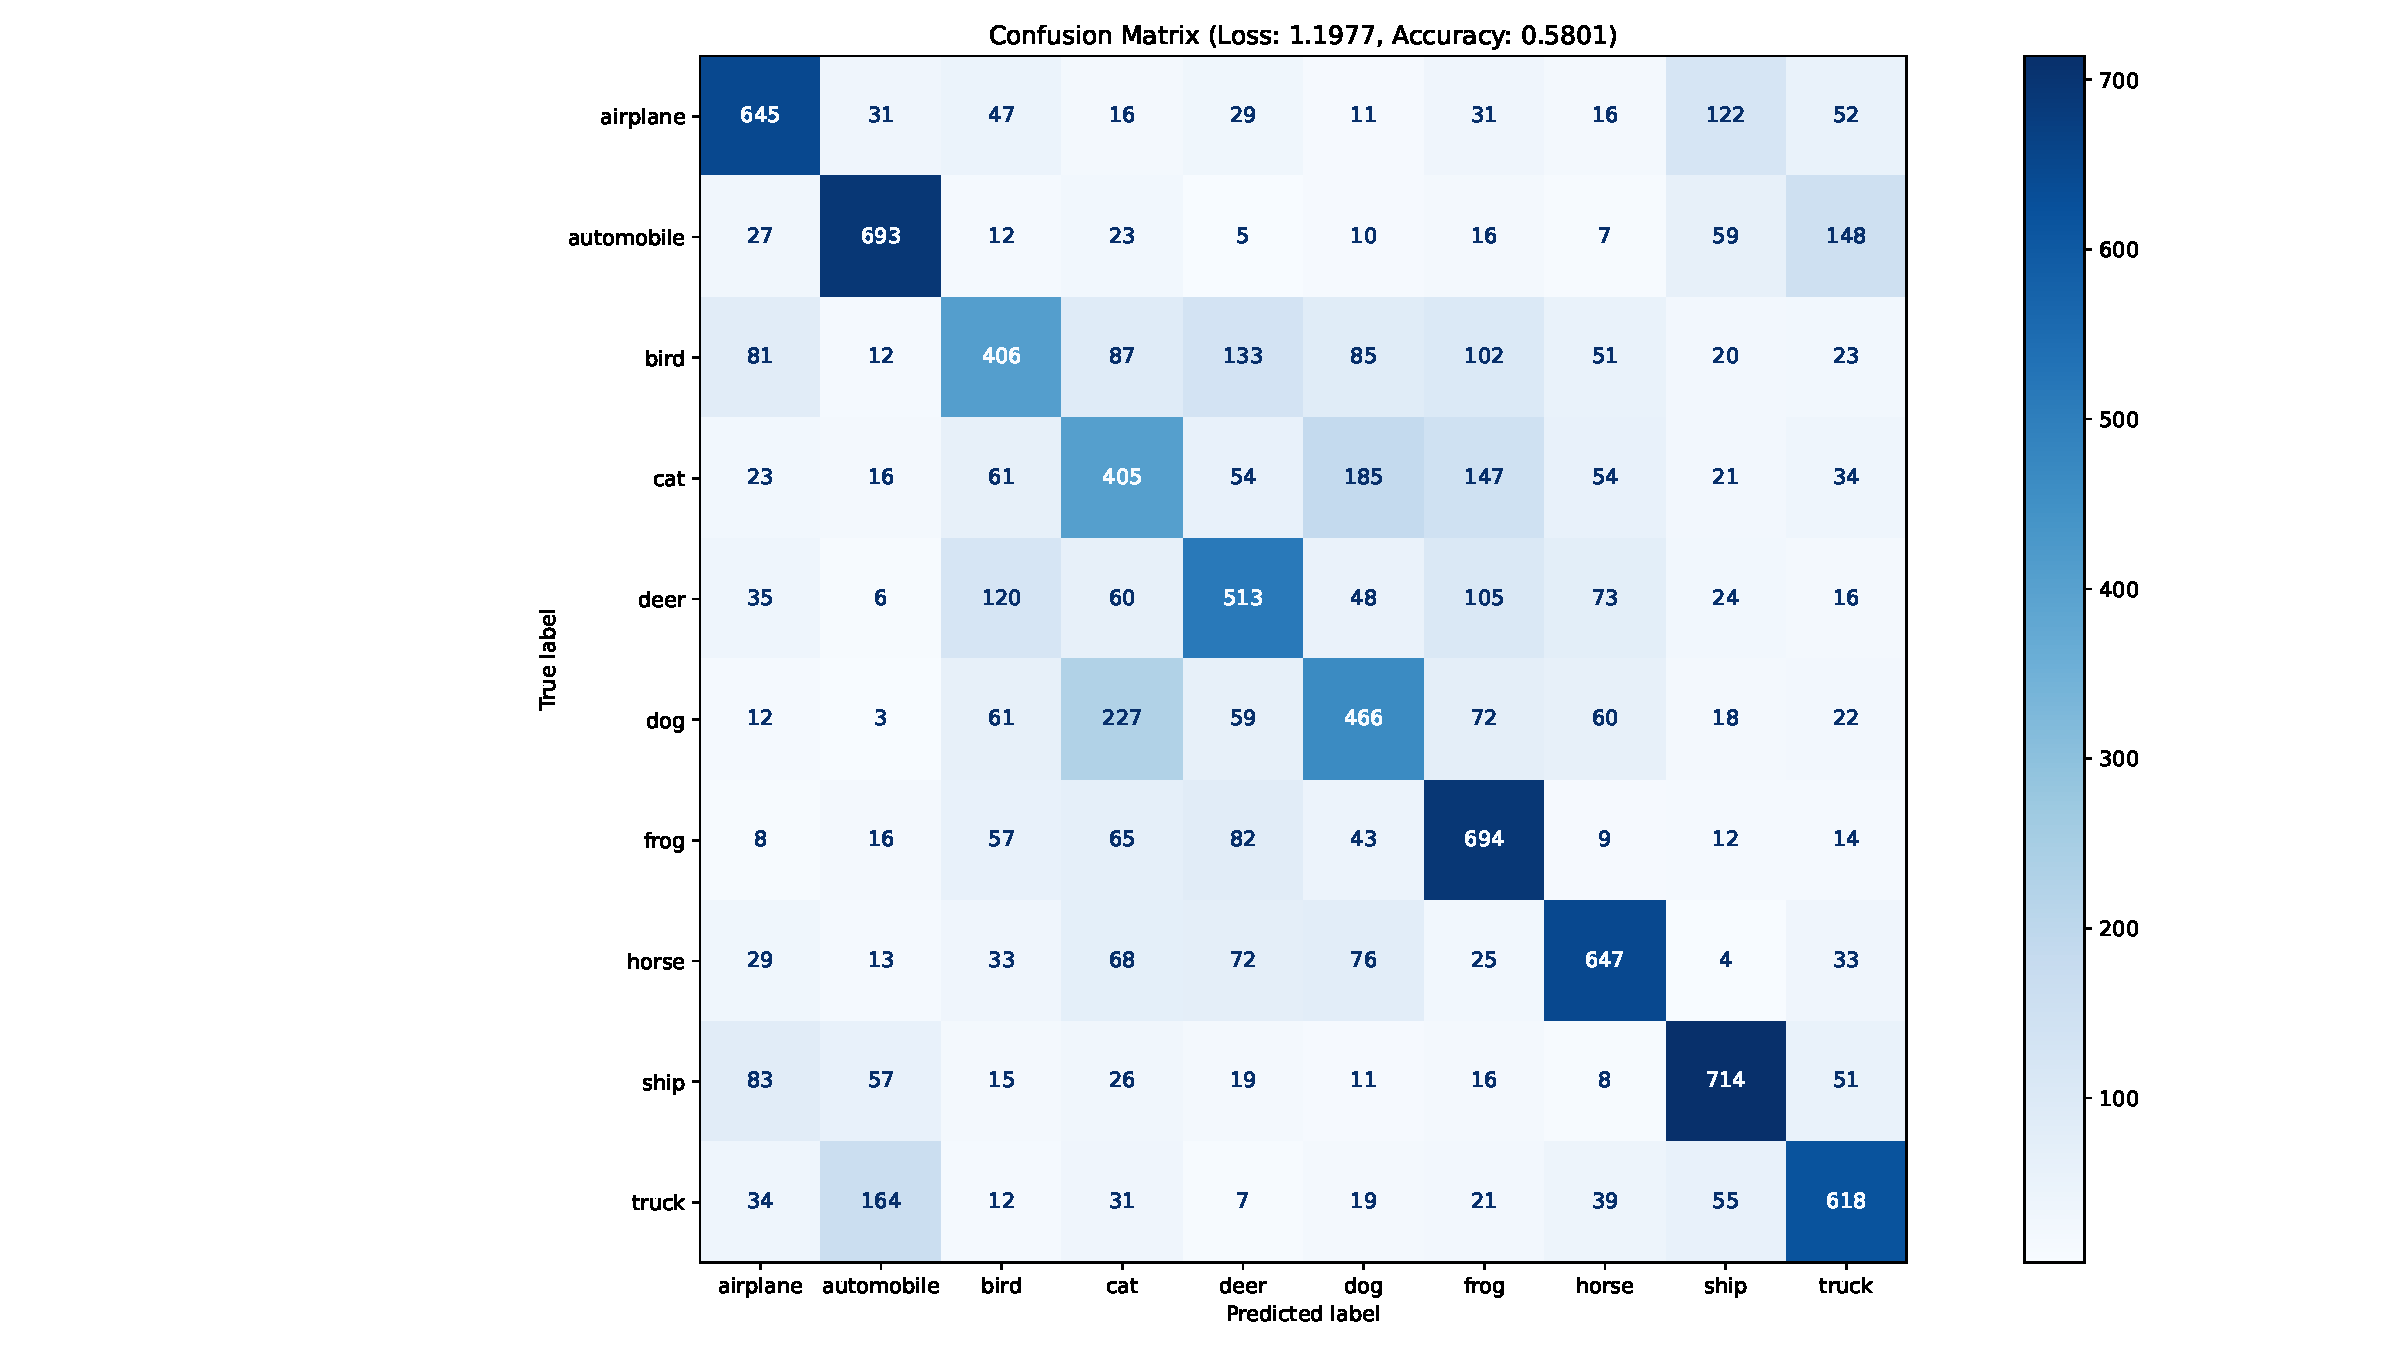
\includegraphics[scale=0.385]{../output/mlp-confusion-matrix.pdf}
    \caption{mlp-confusion-matrix.pdf}
\end{figure}

\begin{figure}[ht]
    \center
    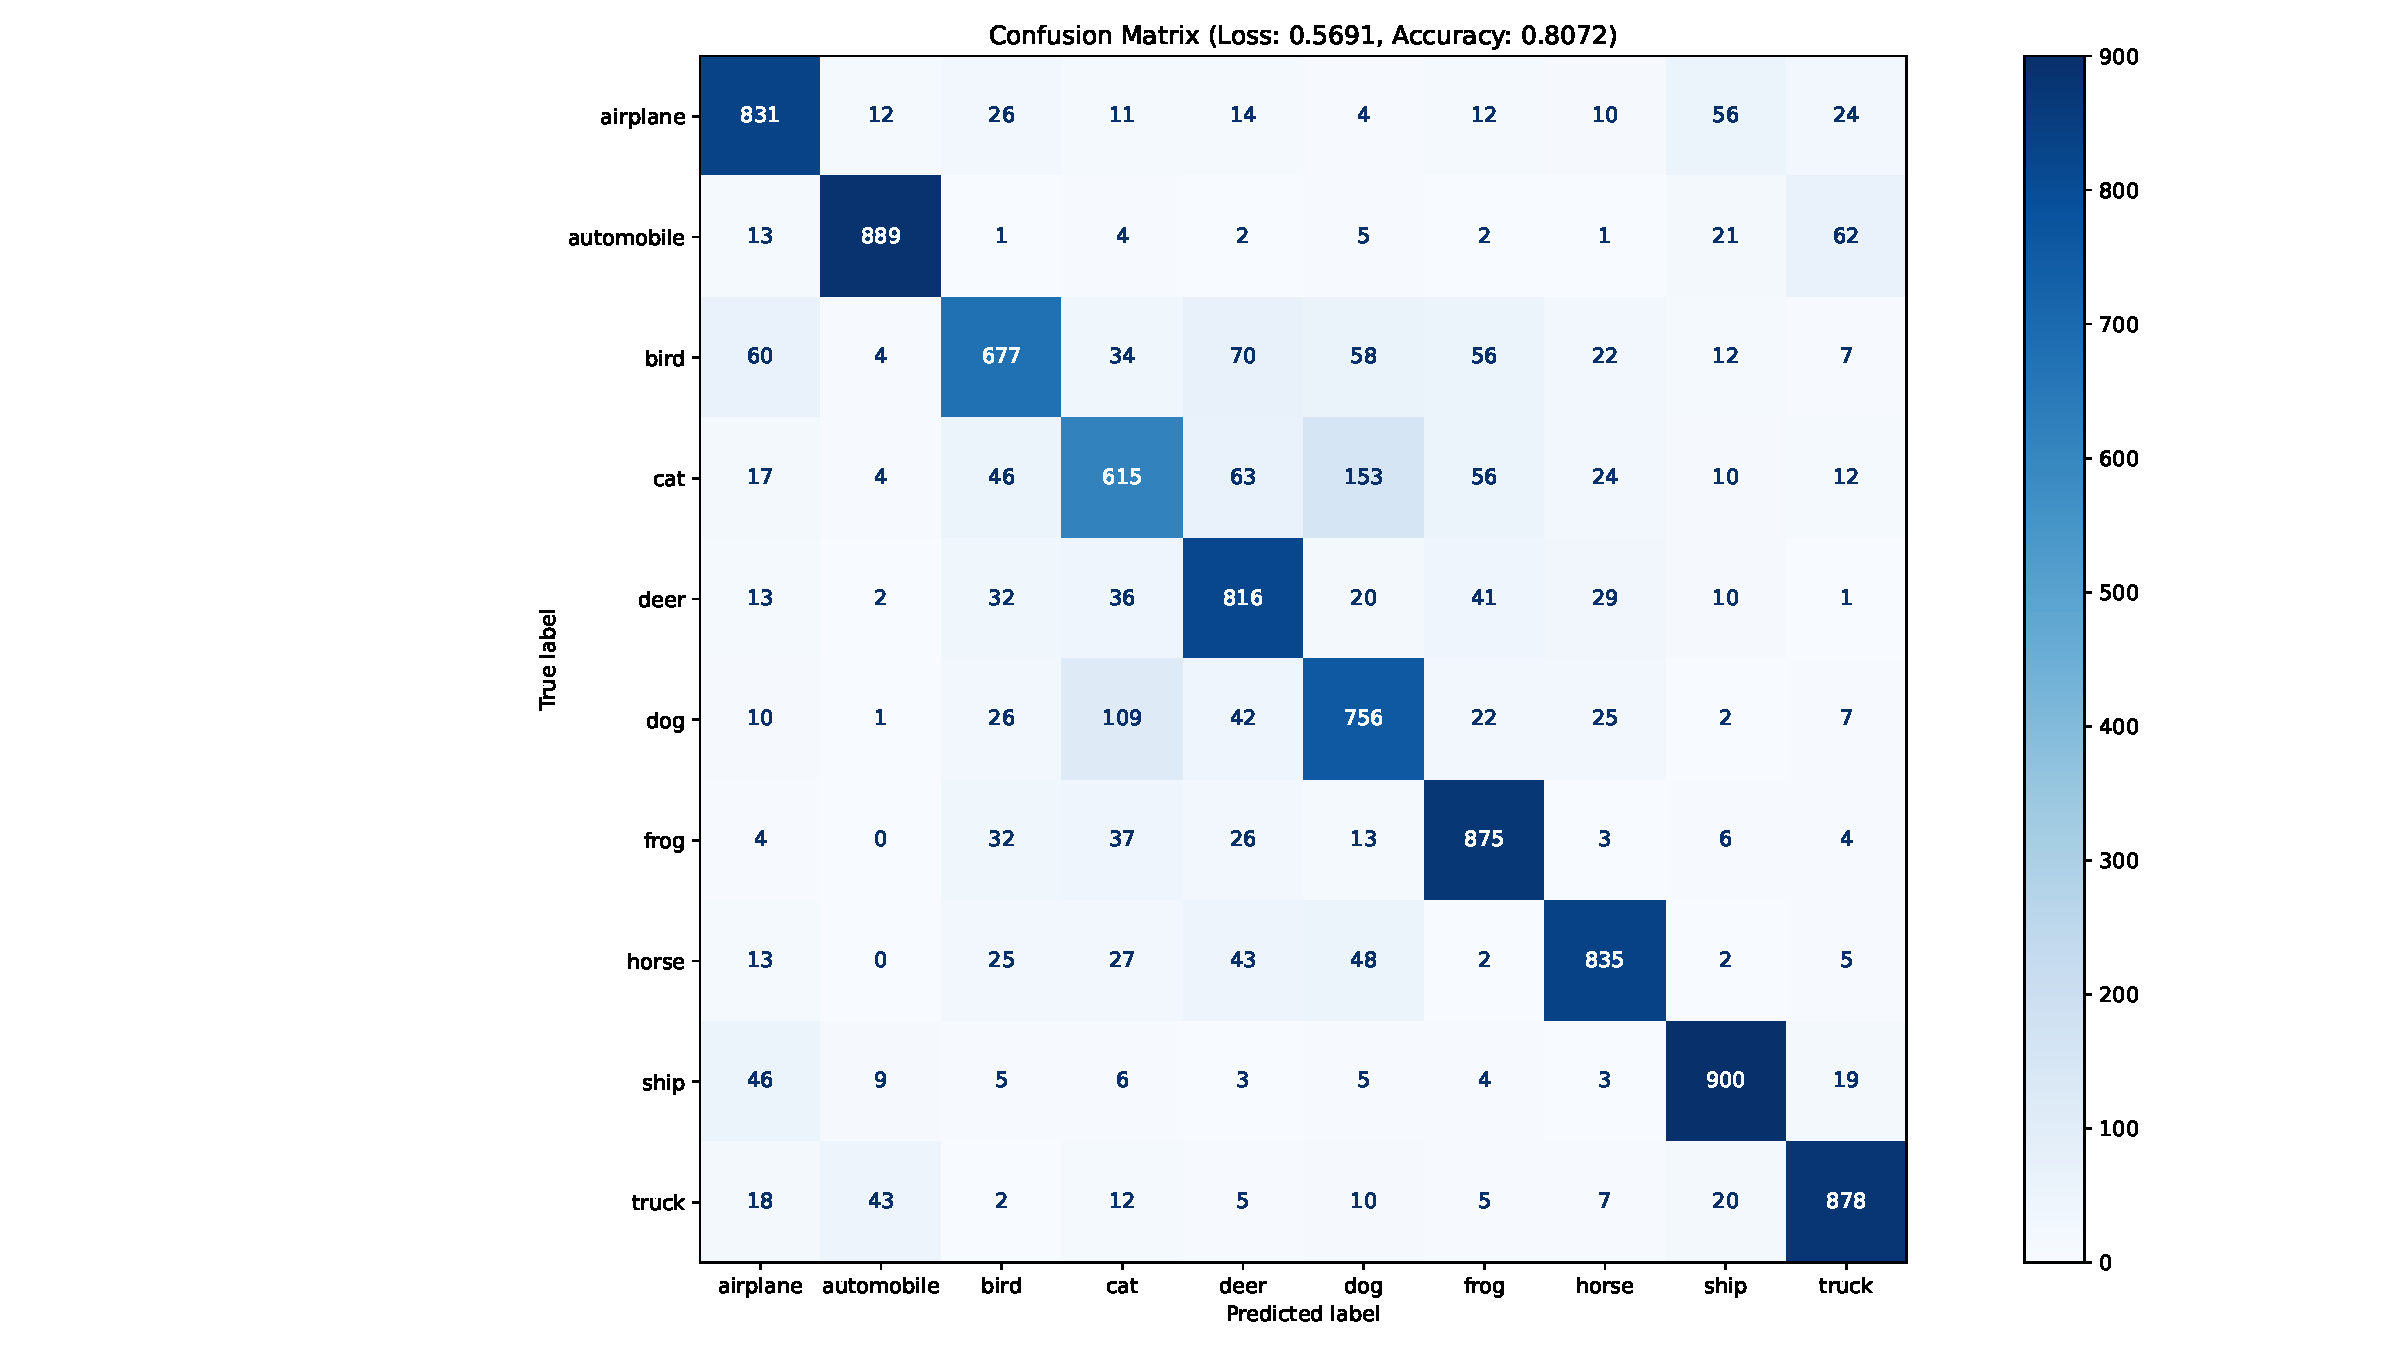
\includegraphics[scale=0.385]{../output/cnn-confusion-matrix.pdf}
    \caption{cnn-confusion-matrix.pdf}
\end{figure}

\section{Discussion}
The two models has an average preformance for any MLPs and CNNs. There are more improvements to be done 
on tuning the models and optimizer parameters, as well as the training and validation method. 

One of the simplest way is to try a wide range of values, since the best parameters might be the least 
expected ones. This method is commonly known as Grid Search, a brute force method to validate each and 
every combinations. But considering the exhaustiveness and inefficient of this, another popular method is 
Random Search - randomly selects a combination. This strange but suprisingly effective method more often 
than not can actually find the best combination. Additionally, because of its lighter weight, more values
can be fitted into the grid to try out even more combinations.

The next thing to consider is the training/validation method. Despite performing well in this project, splitting 20/%
training dataset solely for validating is not the best method. A much better one is doing Cross Validation, 
which is spliting the training set into k folds with equal sizes and in each iteration, one fold is picked for
validation and $k-1$ other folds are for training. After finding the best parameters based on the validation results,
all folds can be used for training.

The last one is to have a learning rate scheduler to adjust the learning rate during training. At the begining the learning 
rate can be setted higher for faster learning. After a few epoch cycle with some signs of slow improvement, the scheduler can 
automatically lowering the learning rate.

\begingroup
\let\clearpage\relax

\chapter*{Conclusion}
Overall, this exercise is a fun way to get introduced into the world of Neural Network. Experimenting with 
architectures like MLP and CNN, loss functions is like a creative playground for solving real-world problems.
Changing a hyperparameter, adjust the architecture, or try a new batch size and immediately see the impact 
feels like building a nonexistent machine to come to life. On the other side, it also shows the short comings
of machine learning when it comes to non linear task like image classification. That's why many CAPTCHA - 
Completely Automated Public Turing Test to tell Computers and Humans Apart - tests use image classification
to detect bots.

\endgroup


% I Want to Be Cold

\end{document}